% arXiv: force the pdflatex path. All content is text, tables and PDF figures; there are no
% .eps files (figures are PDF), and this must stay within the first few lines to take effect.
\pdfoutput=1
\PassOptionsToPackage{hyphens}{url}

\documentclass[11pt]{article}

\usepackage[utf8]{inputenc}
\usepackage[T1]{fontenc}
\usepackage[margin=1in]{geometry}
\usepackage{mathptmx}
\usepackage[scaled=0.92]{helvet}
\usepackage{courier}
\usepackage{amsmath,amssymb,amsthm,mathtools}
\usepackage[numbers,sort&compress]{natbib}
\usepackage{booktabs}
\usepackage{array}
\usepackage{tabularx}
\usepackage{float}
\usepackage{graphicx}
\usepackage{longtable}
\usepackage{enumitem}
\usepackage{caption}
\usepackage{microtype}
\usepackage{xcolor}
\usepackage{tcolorbox}
\tcbuselibrary{breakable}
\usepackage[colorlinks=true,linkcolor=blue!60!black,citecolor=blue!60!black,urlcolor=blue!60!black,breaklinks]{hyperref}
\usepackage{url}
\def\UrlBreaks{\do\/\do-\do.\do\_\do\a\do\b\do\c\do\d\do\e\do\f\do\g\do\h\do\i\do\j\do\k\do\l\do\m\do\n\do\o\do\p\do\q\do\r\do\s\do\t\do\u\do\v\do\w\do\x\do\y\do\z}
\newcommand{\cmd}[1]{\texttt{#1}}
\usepackage{fancyhdr}

\hypersetup{
  pdftitle={The AI-Level Index v2: a harness-standardized capability scale, and the conditions under which an index means anything},
  pdfauthor={Chengshuai Yang},
  pdfsubject={A validated latent capability index for AI models and agents},
  pdfkeywords={capability index, item response theory, leaderboard resolution, anchoring, saturation, false completion}
}

\pagestyle{fancy}
\fancyhf{}
\fancyhead[L]{\small The AI-Level Index v2}
\fancyhead[R]{\small Yang}
\fancyfoot[C]{\thepage}
\renewcommand{\headrulewidth}{0.3pt}
\setlength{\headheight}{14pt}

\definecolor{navy}{HTML}{17324D}
\definecolor{bluec}{HTML}{2B6CB0}
\definecolor{greenc}{HTML}{3A7D44}
\definecolor{orangec}{HTML}{C05621}
\definecolor{lightblue}{HTML}{EAF2F8}
\definecolor{lightgreen}{HTML}{EDF7ED}
\definecolor{lightorange}{HTML}{FFF4E6}

\newcolumntype{Y}{>{\raggedright\arraybackslash}X}
\newcolumntype{Z}{>{\raggedright\arraybackslash\small}X}
\setlist{itemsep=2pt,parsep=0pt,topsep=4pt}
\renewcommand{\arraystretch}{1.15}

\newtheorem{proposition}{Proposition}
\newtheorem{corollary}{Corollary}
\theoremstyle{definition}
\newtheorem{definition}{Definition}

\newtcolorbox{claimbox}[1]{breakable,colback=lightgreen,colframe=greenc,boxrule=0.7pt,arc=2pt,left=7pt,right=7pt,top=6pt,bottom=6pt,title=\textbf{#1},fonttitle=\normalsize,before skip=8pt,after skip=8pt}
\newtcolorbox{cautionbox}[1]{breakable,colback=lightorange,colframe=orangec,boxrule=0.7pt,arc=2pt,left=7pt,right=7pt,top=6pt,bottom=6pt,title=\textbf{#1},fonttitle=\normalsize,before skip=8pt,after skip=8pt}
\newtcolorbox{addedbox}[1]{breakable,colback=lightblue,colframe=bluec,boxrule=0.7pt,arc=2pt,left=7pt,right=7pt,top=6pt,bottom=6pt,title=\textbf{#1},fonttitle=\normalsize,before skip=8pt,after skip=8pt}

\newcommand{\Om}{\ensuremath{\Omega}}
\newcommand{\SA}{\ensuremath{S_A(T,H)}}
\newcommand{\FA}{\ensuremath{F_A(H,p)}}
\newcommand{\rhov}{\ensuremath{\rho_V}}
\begin{document}
\begin{center}
{\LARGE\bfseries The AI-Level Index}\\[6pt]
{\large\bfseries A harness-standardized capability scale, with the estimator validated\\[2pt]
and the cost of a rank measured}\\[14pt]
{\large Chengshuai Yang$^{1,*}$ \quad Ting Xue$^{1}$}\\[5pt]
{\normalsize $^{1}$NextGen PlatformAI C Corp, USA}\\[4pt]
{\normalsize $^{*}$Correspondence: \href{mailto:spiritai@platformai.org}{spiritai@platformai.org}}\\[10pt]
{\small September 6, 2026 --- version 2. Supersedes the v1.1 draft, whose architecture it keeps and whose central weakness it repairs: v1.1 proposed a latent scale and reported that its own fit was degenerate. This version measures what the scale requires.}
\end{center}

\begin{abstract}
Public model comparison runs on composite indices. They are useful because one number can be read, and they share four failures: component benchmarks saturate and are swapped, which breaks the meaning of last year's score; a confident wrong answer costs a model nothing; the number is a property of the model \emph{and} the harness it was measured through, and the harness half is usually undeclared; and the ranks they print are finer than the evidence supports. The AI-Level Index is a public scale built on the AI-Level framework and its benchmark, in which capability levels are invariant by construction and a delivered wrong answer is priced below a declared inability. This paper does something an index paper is not usually asked to do: it measures its own instrument. Six studies on populations with known truth establish what the scale needs before a number from it should be published. \textbf{Recovery}: the ordering is recoverable from a few hundred binary witnesses, but the interval, not the ordering, is what a small population lacks. \textbf{Resolution}: the evidence needed to separate \emph{neighbouring} models grows as the square of the number of models ranked --- measured exponent $2.4$, from $128$ items to distinguish four models to $4096$ for sixteen --- which is why a dense leaderboard that prints ranks is printing noise, and why this index publishes statistically indistinguishable \emph{bands}. \textbf{Anchoring}: when a stronger cohort arrives, free recalibration moves the previous cohort's published scores by $-0.53$ logits systematically, while frozen anchors move them by $-0.006$, inside the $0.33$ standard error; historical comparability is an estimation policy, not a promise. \textbf{Saturation}: as the frontier advances three logits, a fixed suite's bounded composite loses more than half its spread and a third of models reach its ceiling, while witnesses refreshed within fixed levels hold both --- the simulated form of an event this benchmark already had, when two models a tenfold cost apart both scored the instrument's ceiling and four harder witnesses restored a 46-point spread. \textbf{Pricing}: on $38.5\%$ of a competence-by-discrimination grid, a success-only score ranks a bluffing system at or above one that declines what it cannot do, and the delivered-outcome primitive reverses it; the primitive is the linear proxy for what a delegated failure costs. \textbf{Coverage}: partial coverage is survivable and disjoint coverage is not --- linking needs common items, not complete ones. The rapid tier is implemented and has three rows; the latent tier is implemented, and this paper says exactly how many models and witnesses it needs before its numbers should be printed. The claim is not that this index is already better than the incumbents. It is that these are the questions any index must answer, that they are answerable, and that here they are answered.
\end{abstract}

\noindent\textbf{Keywords:} capability index; item response theory; leaderboard resolution; anchoring and equating; benchmark saturation; false completion; harness gain; delegation frontier; measurement validity

\tableofcontents
\bigskip

\section{Introduction}\label{sec:intro}

A capability index compresses many evaluations into one number so that models can be ranked, progress tracked and results communicated. The Artificial Analysis Intelligence Index and the Epoch Capabilities Index both do this, both are independently run, and both report uncertainty \citep{aa2026index, epoch2026eci}. This paper is not an argument that they are wrong. It is an argument that the questions which decide whether \emph{any} such number is worth printing are rarely asked, that they have answers, and that the answers change what a leaderboard should look like.

Four problems recur. First, \textbf{saturation}: when a component benchmark stops separating models it is swapped out, and the index's meaning changes with it; AAI v4.2 removed GPQA Diamond as saturated and doubled its private held-out weight, which is a reasonable maintenance decision and also an admission that discrimination on a fixed mixture decays. Second, \textbf{a wrong answer is free}: almost every component scores accuracy, so a system that guesses confidently outscores one that declines what it cannot do, although the second is the one you can delegate work to. Third, \textbf{the harness is undeclared}: a model's score is a property of the pair (model, harness), and the pair's second half --- retries, tools, memory, acceptance checks --- is usually chosen by whoever ran the evaluation and not reported. Fourth, and least discussed, \textbf{the ranks are finer than the evidence}: leaderboards print an ordered list, and neighbouring entries are typically separated by less than their own uncertainty.

The framework this index sits on \citep{yang2026unified} addresses the first three by construction: levels are stated as contrasts that must hold rather than as difficulty thresholds, so a level cannot be saturated into a different meaning; the delegation primitive is the delivered outcome, so a false completion is charged; and the model is measured through a published ladder of reference harnesses rather than at one undeclared point. The benchmark \citep{yang2026hilbenchpaper} implements them. What neither supplies is evidence about the \emph{index} as an instrument, and that is this paper's subject.

\subsection{What this paper adds}
\begin{enumerate}[leftmargin=*,itemsep=2pt]
\item \textbf{A validated estimator.} The latent scale is fitted on simulated populations with known abilities, and its recovery, interval width and coverage are reported as functions of how many models and how many witnesses are available (\S\ref{sec:recovery}). The v1.1 draft reported that its own fit was degenerate at two models; this paper says what it would take not to be.
\item \textbf{The resolution law.} The item count needed to separate adjacent models grows as $M^{2.4}$ in measurement and as $M^2$ in theory (\S\ref{sec:resolution}). This is a property of ranking under measurement error, not of this index, and it applies to every leaderboard.
\item \textbf{Bands rather than ranks.} The product consequence of the resolution law: report groups whose intervals overlap as one band (\S\ref{sec:bands}), which is both honest and, applied to the three measured rows, immediately informative.
\item \textbf{Anchoring measured, not asserted.} What happens to published scores when a stronger cohort arrives, with and without frozen anchors (\S\ref{sec:anchors}).
\item \textbf{Saturation resistance demonstrated.} A fixed suite and a level-preserving refreshed suite, compared as the frontier advances, in both the bounded-composite and latent readings (\S\ref{sec:saturation}); with the real instance from this benchmark's own history.
\item \textbf{The scoring primitive priced.} The share of parameter space on which a success-only index inverts the ordering a delegator would want, and the cost identity that fixes $\rho$ (\S\ref{sec:bluff}).
\item \textbf{An operational rule for partial coverage.} Which gaps a public index can tolerate and which break the scale (\S\ref{sec:coverage}).
\item \textbf{Three measured rows} on the implemented rapid tier, including a private-split reading and a harness-gain contrast (\S\ref{sec:rapid}).
\end{enumerate}

\subsection{What it does not claim}
It does not claim that the index is already more predictive than the incumbents: the tournament that would settle that is specified (\S\ref{sec:tournament}) and has not been run. It does not claim the latent tier is ready to publish numbers: by its own criterion it is not, and \S\ref{sec:recovery} says what is missing. It does not claim that simulation substitutes for a broad measured population; simulation says what the population must contain.

\section{Relationship to the Existing Indices}\label{sec:related}

\textbf{Artificial Analysis Intelligence Index.} Ten evaluations in four weighted categories, independently run, with cost and speed reported beside intelligence rather than folded into it --- a product principle worth keeping. Its maintenance history is the case for a different design: to keep discriminating, the mixture must change, and when it changes the scale's meaning changes with it.

\textbf{Epoch Capabilities Index.} A latent scale over roughly sixty benchmarks with an item-response model, unbounded, with bootstrap uncertainty and fixed calibration points \citep{epoch2026eci}. ECI is the right response to saturation at the level of \emph{statistics}, and this index does not compete with it by aggregating more benchmarks. Its measurement object is different, and so is the question it can answer.

\textbf{Three questions.} AAI asks how strong a model is on a curated current suite. ECI asks where a model sits on a cross-benchmark latent scale. This index asks \emph{how much verified capability a model realizes as a standardized agent} --- how much can be delegated to it, at what task difficulty, under how much human intervention, with what rate of confidently wrong delivery.

\section{The Measurement Target, and Three Objects That Must Not Merge}\label{sec:target}

The subject is a frozen base model $m$ evaluated through the reference harness family. For a singleton the latent vector is $\Theta_m = [\theta_C, \theta_I, \theta_{DI}, \theta_{SA}]$ --- cognition; persistent individual capability; verified delegation under bounded human intervention; grounded self-modelling and failure recognition. Memory $M$ is certified on its own ladder and reported beside the index rather than inside it, because $I$ already carries the learning and persistence claims and scoring both would count one body of evidence twice.

Three objects must stay distinct. The \textbf{AI-Level} is an ordinal, semantically invariant claim ($U_{I3}$, $C5$, $T4/H1$, $SA3$) earned by canonical evidence with lower-level retention. \textbf{HLIS} is the continuous achievement of one frozen pair. The \textbf{AI-Level Index} is the public, model-level, statistically calibrated comparison scale. \emph{What has been demonstrated; how strong is this pair; where does this base model sit on a common non-saturating scale} --- three questions, three objects, and an index that quietly replaced the first would be the failure this framework exists to avoid.

\section{The Reference Harness Family}\label{sec:harness}

A comparison between base models is only fair if the runtime is standardized, so the index is indexed by a harness family $H^{\mathrm{ref}}_1 = \{\mathrm{HG0}, \ldots, \mathrm{HG6}, \mathrm{HG}\Omega\}$ that fixes context and call budgets, tool and search permissions, persistent-state capacity, the verification and retry interface, time and compute ceilings, the restart mechanism, the human-intervention allowance and authority. Three rungs are built and measured: HG0, one attempt through the model's own API with two read-only tools and a single JSON reply; HG1, the family's public checks --- derivable from the visible specification, never from the key --- with a failing delivery held back; HG2, snapshot, restore and retry with the failed check named. A result is written $\mathrm{AILI}_{2}(m; H^{\mathrm{ref}}_1)$, and a construct-relevant change to the harness requires a new version or a demonstration of equivalence.

The rungs are cumulative in the engineering sense only: $\mathrm{HG}_g = \mathrm{HG}_{g-1} + \Delta_g$, a strict mechanism superset, which is what makes a change in the curve between two rungs attributable to one mechanism. An HG4-conformant harness can still carry an $I2$ system: architecture enables a claim and only the model's own campaign earns it.

\section{The Measurement Model}\label{sec:model}

For a binary canonical evidence unit $i$ on coordinate $d$,
\[
P(Y_{mdi} = 1) = \sigma\!\left[a_i(\theta_{md} - b_i)\right],
\]
with $\theta_{md}$ the model's capability on that coordinate, $b_i$ the calibrated difficulty of the unit and $a_i$ its discrimination; version 2 fits the one-parameter form ($a_i = 1$) and reports the two-parameter form as a robustness check. The unit need not be a question: for longitudinal coordinates it is a whole campaign, and the calibrated observation is whether the campaign's gate closed.

Estimation is joint maximum likelihood by alternating Newton steps, with the origin fixed at mean item difficulty, a mild ridge for identifiability at the extremes, standard errors from the observed information, and one deliberate exclusion: a unit that every model passes or every model fails is dropped and counted, because it carries no information about who is stronger and keeping it only shrinks the scale. Level skipping is prevented by the cumulative transformation $q^{*}_{d,k} = \min_{j \le k} q_{d,j}$ on the capability ladders, and by the corresponding typed rules elsewhere --- a frontier over $T$ at fixed $H$ and $p$ for delegation, mechanism nesting for the harness rungs, and no retention at all on the $T$ and $H$ axes, which classify the item and the transcript rather than the system \citep{yang2026unified}.

The headline is $\theta_H(m) = \sum_{d} w_d\,\theta_{md}$ with equal weights in version 2 --- a stated convention, not a finding --- and
\[
\mathrm{AILI}(m) = 100 + s\,\theta_H(m), \qquad s = 10,
\]
unbounded above and below, so that a frontier advance moves models up the scale instead of compressing them against a ceiling. For a bare model $\theta_I$ is not estimable ($I0$ by construction) and the weights are renormalized over the coordinates present, which the record states.

\section{Six Studies of the Instrument Itself}\label{sec:studies}

Everything above is design. What follows is measurement, on populations where the truth is known by construction, so that the estimator can be scored against it. All six studies are in \texttt{hilbench/index\_sim.py}, run by one command, and the tables and figures below are generated from the run they write; a test asserts that the fast estimator used here agrees with the package's canonical one on a shared case, so speed does not buy a different answer.

\subsection{Recovery: what the estimator needs}\label{sec:recovery}

Simulate $M$ models with abilities drawn from a unit normal and $K$ witnesses with difficulties drawn from $\mathcal N(0, 1.2)$, generate responses under the model, fit, and compare with the truth. Table~\ref{tab:sample} reports three numbers per cell: the rank correlation, the share of \emph{adjacent} pairs whose 95\% intervals do not overlap, and the median standard error in logits (one logit is ten index points).

\begin{table}[!htbp]\centering\small
\begin{tabular}{@{}lcccc@{}}\toprule
$M$ & $K=40$ & $K=80$ & $K=160$ & $K=320$ \\ \midrule
2 & 1.00 / 1.00 / 0.61 & 1.00 / 1.00 / 0.41 & 1.00 / 1.00 / 0.31 & 1.00 / 1.00 / 0.19 \\
3 & 1.00 / 0.00 / 0.47 & 1.00 / 0.50 / 0.35 & 1.00 / 0.50 / 0.24 & 1.00 / 0.50 / 0.16 \\
5 & 0.90 / 0.00 / 0.44 & 0.90 / 0.25 / 0.30 & 1.00 / 0.50 / 0.21 & 1.00 / 0.50 / 0.15 \\
8 & 0.83 / 0.00 / 0.40 & 0.93 / 0.00 / 0.29 & 0.95 / 0.14 / 0.20 & 0.98 / 0.29 / 0.14 \\
12 & 0.92 / 0.00 / 0.39 & 0.94 / 0.00 / 0.28 & 0.97 / 0.09 / 0.20 & 0.98 / 0.14 / 0.14 \\
20 & 0.94 / 0.00 / 0.39 & 0.96 / 0.00 / 0.27 & 0.97 / 0.00 / 0.19 & 0.99 / 0.11 / 0.13 \\
40 & 0.93 / 0.00 / 0.38 & 0.96 / 0.00 / 0.27 & 0.98 / 0.00 / 0.19 & 0.99 / 0.03 / 0.13 \\
\bottomrule\end{tabular}
\caption{Recovery against known truth: Spearman correlation / share of adjacent pairs separated at 95\% / median standard error, at $M$ models and $K$ witnesses, median over 30 replications. Spearman is uninformative below about eight models --- with two or three, any estimator orders them almost surely --- which is why the middle number matters more.}
\label{tab:sample}
\end{table}

Two readings. First, \emph{the ordering is cheap and the interval is not}: rank correlation passes $0.95$ at 160 witnesses and stays there, while the standard error falls only as $1/\sqrt{K}$, from $0.39$ logits at $K=40$ to $0.13$ at $K=320$ --- from $\pm 7.6$ to $\pm 2.6$ index points at 95\%. An index published from a small evidence base can say who is ahead and cannot say by how much. Second, and less comfortable, \emph{adjacent separation falls as the population grows}: at four models and 320 witnesses half of neighbouring pairs are distinguishable; at forty models, three per cent are. Nothing is wrong with the estimator. The gaps between neighbours shrink faster than the errors do.

\subsection{The resolution law: what a rank costs}\label{sec:resolution}

That observation has a form. For $M$ abilities drawn from a unit normal, the typical gap between neighbours near the middle of the distribution is about $\sqrt{2\pi}/M \approx 2.5/M$. Separating two estimates at 95\% requires their gap to exceed $1.96\sqrt2\,\mathrm{SE} \approx 2.77\,\mathrm{SE}$, so
\[
\mathrm{SE} \lesssim \frac{0.9}{M}, \qquad \text{and since } \mathrm{SE} \approx \frac{2}{\sqrt K}, \qquad K \gtrsim 5 M^2 .
\]
Doubling the number of models a leaderboard wants to \emph{rank} quadruples the evidence each model must supply. Figure~\ref{fig:resolution} scans for the smallest $K$ at which half of adjacent pairs separate: 128 witnesses for four models, 512 for six, 1024 for eight, 2048 for twelve, 4096 for sixteen, a log--log slope of $2.4$. The exponent exceeds the idealized $2$ because item difficulties are spread rather than matched to the population and uninformative items are dropped; the constant is larger for the same reason.

\begin{figure}[!htbp]\centering
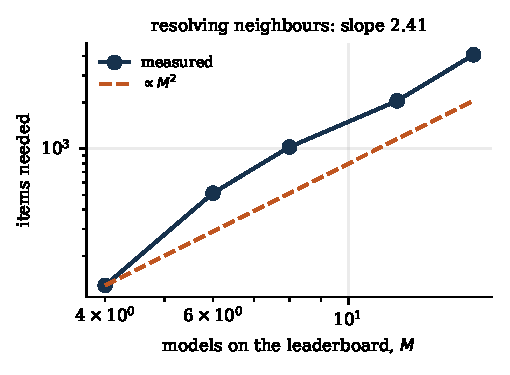
\includegraphics{fig_resolution.pdf}
\caption{The item count needed before half of adjacent models are separated at 95\%, against the number of models ranked, with the $M^2$ reference. Ranking is quadratically more expensive than scoring.}
\label{fig:resolution}
\end{figure}

This is a property of ranking under measurement error and applies to every leaderboard, including the incumbents; it is stated here because an index that prints a hundred ordered rows is making a claim about resolution that no feasible evidence base supports. The right response is not more items. It is to stop printing a rank the evidence cannot carry.

\subsection{Bands, not ranks}\label{sec:bands}

The index therefore publishes \emph{bands}: models are ordered by $\mathrm{AILI}$, and consecutive models whose 95\% intervals overlap are printed as one statistically indistinguishable group (\texttt{index\_sim.bands}). Within a band there is no order to report. A band boundary is a claim the evidence supports, and a rank inside a band is not. This costs nothing that was real and removes the part of a leaderboard that is most often over-read --- and it makes the index's uncertainty visible in the artefact people actually look at, rather than in a column they skip.

\subsection{Anchors, and whether last year's score still means anything}\label{sec:anchors}

A published index number must keep its meaning when the next cohort arrives. Simulate eight models measured on an anchor set; then add eight stronger models, measured on the anchors plus fresh witnesses whose difficulty tracks the new frontier, and ask what happened to the first cohort's published scores.

\begin{table}[!htbp]\centering\small
\begin{tabular}{@{}lcc@{}}
\toprule
Calibration policy & Systematic drift (logits) & Absolute drift (logits) \\
\midrule
Free recalibration over all data & $-0.53$ & $0.57$ \\
Frozen anchors carry the scale & $-0.01$ & $0.36$ \\
\midrule
\multicolumn{3}{@{}l}{\emph{measurement noise for reference: median SE $= 0.33$ logits}} \\
\bottomrule
\end{tabular}
\caption{What adding a stronger cohort does to the previous cohort's published scores, median over 30 replications. Absolute drift mixes noise with bias; the signed drift is the bias. Under free recalibration the first cohort loses half a logit --- five index points --- for no reason connected to its own capability. Under frozen anchors the movement is indistinguishable from noise.}
\label{tab:equating}
\end{table}

Free recalibration is the natural thing to do and it silently rewrites history: the origin follows the mean difficulty of whatever items are in the pool, so adding harder items for a stronger cohort pushes everyone already on the board downwards. Frozen anchors --- a permanent set whose difficulties are fixed after ratification, with new witnesses calibrated against them --- remove the bias entirely. The operational rule follows: publish a \emph{frozen historical} index that is never recomputed under the same version, and, if a current-fit view is wanted, publish it separately and label it a diagnostic.

\subsection{Saturation: a fixed suite stops measuring}\label{sec:saturation}

Let the frontier advance by $0.6$ logits a year for five years and compare two suites: one fixed at its year-zero difficulties, and one whose witnesses are refreshed within fixed levels so that difficulty tracks the population --- which is what ``saturation motivates harder witnesses, not a redefined level'' means when it is implemented.

\begin{table}[!htbp]\centering\small
\begin{tabular}{@{}lcccccc@{}}\toprule Frontier & \multicolumn{3}{c}{bounded composite} & \multicolumn{2}{c}{separation} & at ceiling \\ \cmidrule(lr){2-4}\cmidrule(lr){5-6}
(logits) & mean, fixed & spread, fixed & spread, refreshed & fixed & refreshed & fixed \\ \midrule
0.0 & 0.52 & 0.162 & 0.176 & 0.96 & 0.96 & 0.00 \\
0.6 & 0.58 & 0.167 & 0.174 & 0.97 & 0.96 & 0.00 \\
1.2 & 0.70 & 0.147 & 0.168 & 0.95 & 0.96 & 0.00 \\
1.8 & 0.76 & 0.133 & 0.181 & 0.95 & 0.97 & 0.00 \\
2.4 & 0.86 & 0.085 & 0.166 & 0.92 & 0.96 & 0.17 \\
3.0 & 0.91 & 0.074 & 0.184 & 0.87 & 0.97 & 0.33 \\
\bottomrule\end{tabular}
\caption{The frontier advances three logits. The fixed suite's bounded composite rises from $0.52$ to $0.91$ and its spread across models collapses from $0.162$ to $0.074$, with a third of models at its ceiling; the refreshed suite holds both its spread and its separation reliability. Median over replications.}
\label{tab:saturation}
\end{table}

\begin{figure}[!htbp]\centering
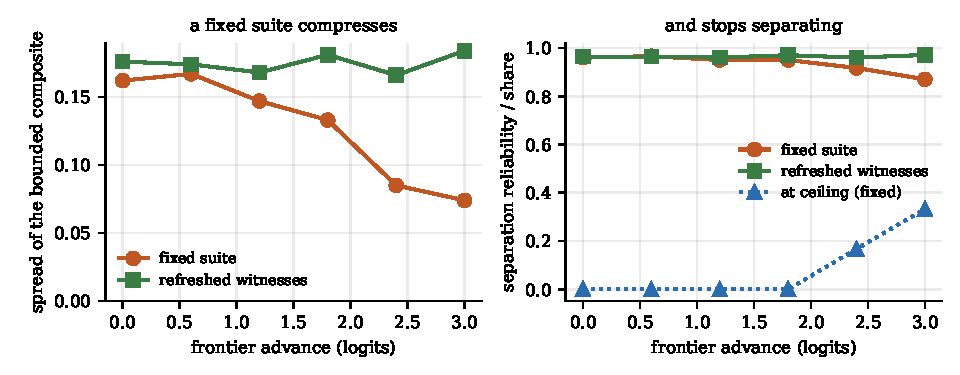
\includegraphics{fig_saturation.pdf}
\caption{Left: the spread of a bounded composite --- the AAI-shaped quantity --- against frontier advance, for a fixed and a refreshed suite. Right: separation reliability, and the share of models at the fixed suite's ceiling.}
\label{fig:saturation}
\end{figure}

Two things are worth separating. The bounded composite degrades \emph{fast}: more than half its spread is gone after three logits, which is what forces a maintained index to swap components. The latent fit on the same fixed suite degrades more gracefully ($0.96 \to 0.87$ separation) because it estimates ability rather than averaging scores --- an argument for ECI's approach over a weighted mean --- but it degrades, and a third of models sitting at the ceiling of every item is a limit no estimator can see past.

The benchmark this index sits on has already run the experiment for real. On its Core, two models a tenfold cost apart both scored $90.0$ --- the instrument's ceiling, not theirs. Four harder witnesses were designed, calibrated against both pairs and admitted only after a program verified each satisfied its level's law; with them the same two models separated by 46 points. No level changed meaning in the process, which is the whole point: the level said what it always said, and the witness got harder.

\subsection{Pricing a bluff}\label{sec:bluff}

Consider two systems of equal underlying competence $q$. One attempts everything. The other declines what it judges it cannot do, with some skill at telling its failures from its successes, and occasionally declines something it would have got right. Under a success-only score the second is punished for every refusal. Under the delivered-outcome primitive
\[
S_{\mathrm{net}} = P(\text{delivered} \wedge \text{verified}) - \rho\,P(\text{false completion}),
\]
a refusal costs nothing and a confident wrong delivery costs $\rho$. Across a grid of competence and discrimination, \textbf{on $38.5\%$ of cells a success-only index ranks the bluffing system at least as high while the delivered-outcome primitive prefers the system that declines}. That is not a corner case; it is more than a third of the plausible parameter space, and it is the region where the two indices would give a buyer opposite advice.

The choice of $\rho$ is not arbitrary. If a wrong delivery costs the delegator $c_{\mathrm{wrong}}$ --- the work of detecting it, plus whatever it caused downstream --- and a held-back task costs $c_{\mathrm{redo}}$ to route elsewhere, then expected cost is $c_{\mathrm{wrong}}P(\text{false completion}) + c_{\mathrm{redo}}P(\text{held back})$, and $S_{\mathrm{net}}$ is its linear proxy at $\rho = c_{\mathrm{wrong}}/c_{\mathrm{redo}}$. The ratified $\rho = 1$ is the statement that an undetected wrong answer costs about what redoing the task costs; in domains where it costs more, the standard's constant is the thing to change, and changing it changes the version.

\subsection{Coverage: linking needs common items, not complete ones}\label{sec:coverage}

A public index will never have every model on every witness: labs run the cheap tier, some models lack a modality, campaigns are expensive. Which gaps are survivable?

\begin{table}[!htbp]\centering\small
\begin{tabular}{@{}lccc@{}}\toprule Coverage & Spearman & median SE & SE, partial models \\ \midrule
complete & 0.965 & 0.19 & 0.19 \\
missing at random, 40% & 0.951 & 0.26 & 0.26 \\
blocked by difficulty, items shared & 0.965 & 0.24 & 0.28 \\
disjoint: the halves share no item & 0.853 & 0.29 & 0.30 \\
\bottomrule\end{tabular}
\caption{Ordering recovery and interval width under four coverage regimes, twelve models and 160 witnesses. ``SE, partial models'' is the interval on the models that skipped part of the suite.}
\label{tab:coverage}
\end{table}

The result corrects an intuition, including the one this paper's authors started with. Blocked coverage --- half the models running only the easy half of the suite --- costs almost nothing in ordering ($0.965$, against $0.965$ complete), because the hard witnesses are still answered by the other half and carry the scale; the models that skipped are placed with a \emph{wider interval} ($0.28$ against $0.19$), which is the correct behaviour: less evidence, less confidence, not a confident wrong number. What breaks the scale is \emph{disjoint} coverage, where the two halves of the population share no witness at all: ordering falls to $0.85$ and the two halves are no longer on one scale in any meaningful sense. Hence the operational rule: \textbf{every published row must share a minimum set of anchor witnesses with every other}, and a tier that shares nothing with the tier above it is a separate scale wearing the same name.

\section{The Rapid Tier, and Three Measured Rows}\label{sec:rapid}

Until a weak-to-frontier population exists, the latent tier cannot be calibrated --- and by \S\ref{sec:recovery}'s own criterion, publishing its numbers from two or three models would be publishing an interval wider than the scale. The rapid tier is what runs today: a bounded composite over the three built rungs,
\[
\text{AILI}_{\mathrm{rapid}} = 0.55\cdot\mathrm{AUC}_{\mathrm{HG0..HG2}} + 0.35\cdot\mathrm{Ceiling} + 0.10\cdot\mathrm{Harnessability},
\]
about 150 calls and a few minutes for a hosted model, with $\rho = 1$. Its evidence units are a strict subset of the latent tier's, so nothing measured now is discarded when the latent tier is ratified.

\begin{table}[!htbp]\centering\footnotesize
\begin{tabular}{@{}p{3.2cm}p{2.4cm}cccc c>{\raggedright\arraybackslash}p{1.5cm}@{}}\toprule Model & Split & Index & HG0/HG1/HG2 & Gain & FCR & Decl. & Profile \\ \midrule
DeepSeek \texttt{deepseek-chat} & public, 3 seeds/family & \textbf{32.3} & 35.9/35.9/35.9 & 0.0 & 0.00 & 0.06 & C3, SA1, T1 \\
DeepSeek \texttt{deepseek-chat} & private, 4 salt-derived seeds & \textbf{35.2} & 31.3/39.5/39.2 & 8.2 & 0.04 & 0.04 & C3, SA1, T1 \\
Qwen 3.8 27B \texttt{qwen3.8:27b} & public, 3 seeds/family & \textbf{30.3} & 26.1/34.9/31.3 & 8.8 & 0.08 & 0.10 & C3, SA1, T0 \\
\bottomrule\end{tabular}
\caption{Rapid-tier rows, taken by the instrument's author, who built neither model. FCR is the false-completion rate.}
\label{tab:rows}
\end{table}

The rows already show the quantity the framework says should carry information. The smaller model bluffs --- three false completions bare, FCR $0.08$ --- and gains $8.8$ points from a harness that catches part of it. The larger model bluffs nowhere and gains nothing, because a retry loop has nothing to correct. Two models, one lesson, and the first of this paper's falsifiable predictions (\S\ref{sec:predictions}): \emph{harness gain is largest for models whose failures are catchable}. On the private split the DeepSeek row reads $35.2$ against $32.3$ public, a difference well inside the interval that \S\ref{sec:recovery} says three seeds per family buys.

Applying \S\ref{sec:bands} to these three rows puts all of them in one band. That is the honest reading of three rows taken at this evidence level, and it is exactly what a leaderboard should say rather than printing a podium.

\section{Tiers, Uncertainty, and the Validation Program}\label{sec:validation}

An entry is \emph{Preliminary} (core evidence, limited to tested capabilities) or \emph{Certified} (full evidence, private split, independent runner). A preliminary score never infers untested longitudinal capability: a model with no $I$ campaign is $I0$ \emph{by construction}, not by failure, and the record says which. Every score carries an interval; the leaderboard shows bands.

Beyond the six studies here, the program requires: test--retest across independent hidden runs; alternate-form reliability across construct-equivalent generated witnesses; provider stability for the same frozen weights served by different providers; construct validity by mechanism-selective ablation, where ablating a mechanism relevant to one coordinate impairs that coordinate more than the others; and rank robustness under seed-set change. Two of these already have instances in the benchmark's record: the bare DeepSeek row read $35.2$ on both splits once the gating band carried twelve episodes, and a pair's unified level moved from U0 to U1 on that same extension --- which is why intervals at the gating band are a requirement and not a nicety.

\section{The Predictive-Validity Tournament}\label{sec:tournament}

The strongest evidence for an index is external prediction. For models $m = 1..N$ collect $H_m$, $E_m$, $A_m$ --- this index, ECI, AAI --- and an independent downstream suite used to construct none of them: repository-scale software work, research and analysis workflows, document-intensive professional work, long-horizon completion, error recovery, human intervention required, delivered correctness, failure recognition. Compare $\rho(H, Y)$, $\rho(E, Y)$, $\rho(A, Y)$ and the explained variances, with the comparison preregistered and the outcome suite frozen before any index is computed. The hypothesis is specific: the coordinates this index adds --- persistent individual capability, the delegation frontier, and false-completion behaviour --- should predict deployed agent outcomes beyond what a cognition-weighted score explains. If they do not, the extra machinery is not earning its cost, and that is a result worth publishing too.

\section{The Public Product}\label{sec:product}

A technically sound index that covers few models or reports slowly will not be used. The requirements: rapid preliminary evaluation of major releases, which the rapid tier makes a matter of API access; broad provider and open-weight coverage; reproducible model-version identifiers; a public historical time series under frozen anchors; transparent handling of retired models; and a machine-readable API beside the page.

The first view is one number and a band. Beneath it: the interval, $\theta_C$, $\theta_I$, $\theta_{DI}$, $\theta_{SA}$, the harness scaling curve, harness gain, false-completion rate, verification responsiveness, cost, latency, tokens, and the version string. Every official result supports the compact form
\[
\mathrm{AILI} \mid \text{AI-Level} \mid [C, I, T/H, SA] \mid M, \qquad \text{e.g. } 154 \mid U_{I3} \mid [C5, I3, T4/H1, SA3] \mid M4,
\]
and a standalone number is never the complete result. Versioning names the semantic standard, the index version, the harness version and the witness generation (\texttt{AIL-1.0/Index-2.0/HRH-1/2026Q3}); semantic revisions require a new major standard, calibration changes a new index version, and witness renewal neither. Governance separates the party funding an evaluation, the runner, the owner of hidden witnesses, the verifier and the certification authority; payment or participation must not affect tasks, seeds, thresholds, rubrics or calibration.

\section{Falsifiable Predictions}\label{sec:predictions}

\begin{enumerate}[leftmargin=*,itemsep=1pt]
\item Models with similar raw cognition will differ materially in harness gain, and gain will be largest where failures are catchable by a public check.
\item $\theta_I + \theta_{DI}$ will predict long-horizon agent performance better than cognition-only scores.
\item The delegation frontier will predict required human intervention better than generic agent accuracy.
\item False-completion-aware metrics will explain deployment reliability beyond raw success.
\item Construct-equivalent refreshed witnesses will retain discrimination without semantic redefinition, where a fixed suite will not.
\item Under frozen anchors, a model's published index will not move by more than its interval when later cohorts are added.
\item Adjacent leaderboard entries within a band will not be separable by any independent replication at the same evidence level.
\end{enumerate}
Predictions 5, 6 and 7 are already supported in simulation here; supporting them in the field is the next step, and prediction 1 has two measured rows.

\section{Limitations}\label{sec:limits}

The six studies are simulations. They are informative about the estimator and say nothing about whether real models' abilities are unidimensional per coordinate, whether real witnesses fit a one-parameter model, or whether real difficulty distributions look like the ones drawn here; the sample requirements should be read as necessary conditions, not sufficient ones. Three measured rows are not a population, and all three were taken by the instrument's author --- who built neither model, which is weaker than independence but not nothing. Weights and scale are conventions. Coordinate equating must be validated before aggregation is defensible. Upper individual levels need expensive longitudinal evidence. Generators develop artefacts and need auditing. A standardized harness cannot represent every production architecture. Superior conceptual structure demonstrates nothing about practical validity, and this paper deliberately reports the questions it cannot yet answer next to the ones it can.

\section{Roadmap}\label{sec:roadmap}

Freeze the version-2 specification; ratify the permanent anchor set; evaluate a weak-to-frontier population large enough for the latent tier by \S\ref{sec:recovery}'s criterion (of order ten to twenty models, with at least the item count \S\ref{sec:resolution} implies for the bands to mean anything); fit and validate the coordinate scales; run test--retest and alternate-form reliability; release a public beta with bands; run the external tournament; commission an independent audit; ratify version 2 only after the evidence is satisfactory.

\section{Conclusion}

An index is a measurement instrument, and a measurement instrument that has never been measured is a proposal. This paper keeps the architecture that makes the AI-Level Index worth building --- invariant levels, a standardized harness family, a delivered-outcome primitive that prices a bluff, permanent anchors, an unbounded scale --- and adds what was missing: evidence about the instrument. The estimator recovers a known ordering from a few hundred witnesses, and its intervals, not its ordering, are what small evidence bases lack. Ranking neighbours costs quadratically more than scoring them, so the leaderboard publishes bands. Frozen anchors keep published numbers still when the frontier moves, and free recalibration does not. A fixed suite stops measuring as the frontier advances, and refreshed witnesses within fixed levels do not. A success-only score inverts the ordering a delegator wants on more than a third of the plausible parameter space. Partial coverage is survivable, disjoint coverage is not.

None of that makes this index better than the incumbents today; it has three rows and they have hundreds. It does mean that when the rows exist, the number attached to them will have known properties --- which is the only durable case any index can make, and one that can be checked rather than believed.

\appendix
\section{Provisional Specification, Version 2}\label{app:spec}
\begin{itemize}[leftmargin=*,itemsep=1pt]
\item \textbf{Subject.} A frozen model through $H^{\mathrm{ref}}_1$. Pair readings are HLIS and are never index rows.
\item \textbf{Evidence units.} Binary outcomes of canonical witnesses: delegation episodes under the delivered-outcome primitive; cognition items by band, seed and rung; self-awareness probes; and, for agent rows, the $M$, $I$ and organizational campaigns.
\item \textbf{Model.} $P(Y=1) = \sigma[a_i(\theta_{md} - b_i)]$, $a_i = 1$ in version 2; per-coordinate scales; origin at mean anchor difficulty; standard errors from the observed information; uninformative units dropped and counted.
\item \textbf{Headline.} $\theta_H = \sum w_d\theta_{md}$, $w = 1/4$ each, renormalized over the coordinates present; $\mathrm{AILI} = 100 + 10\,\theta_H$; interval $\pm 1.96\,\mathrm{SE}$; published as bands.
\item \textbf{Rapid tier.} $0.55\,\mathrm{AUC} + 0.35\,\mathrm{Ceiling} + 0.10\,\mathrm{Harnessability}$ in $[0,100]$, $\rho = 1$.
\item \textbf{Beside the headline.} AI-Level, $[C, I, T/H, SA]$, $M$, FCR, decline rate, harness gain, delegation frontier, resources, interval, version string.
\item \textbf{Anchors.} A permanent set per coordinate, difficulties frozen after ratification; frozen-historical index published, current-fit view labelled a diagnostic.
\item \textbf{Coverage.} Every row shares the anchor set with every other; a row that shares nothing with the rows above it is not placed on the scale.
\item \textbf{Publication.} Bands, not ranks. A rank inside a band is not reported.
\end{itemize}

\section{Reproduction}\label{app:repro}
\begin{verbatim}
# the six studies, written to records/index_sim/index_sim.json
python3 -c "from pathlib import Path
from hilbench import index_sim as S
S.run_all(Path('records/index_sim'))"

# figures and tables for this paper
python3 tools/index_paper_assets.py records/index_sim ../ail_index_v2

# one rapid-tier row
python3 -m hilbench index --base ENDPOINT --model NAME --root DIR

# the latent fit over every published row
python3 -m hilbench latent --split public

# the estimator's tests, including agreement with the package fitter
python3 -m pytest -q tests/test_index_sim.py
\end{verbatim}

\section*{Availability}
The simulation module, the estimator, the rapid-tier runner, every record and the anchor commitment are in \citet{yang2026hilbench}; the benchmark in \citet{yang2026hilbenchpaper}; the framework in \citet{yang2026unified}.

\section*{Conflicts and funding}
The authors built the instrument and neither model measured. No external funding.

\bibliographystyle{plainnat}
\bibliography{references}
\end{document}
